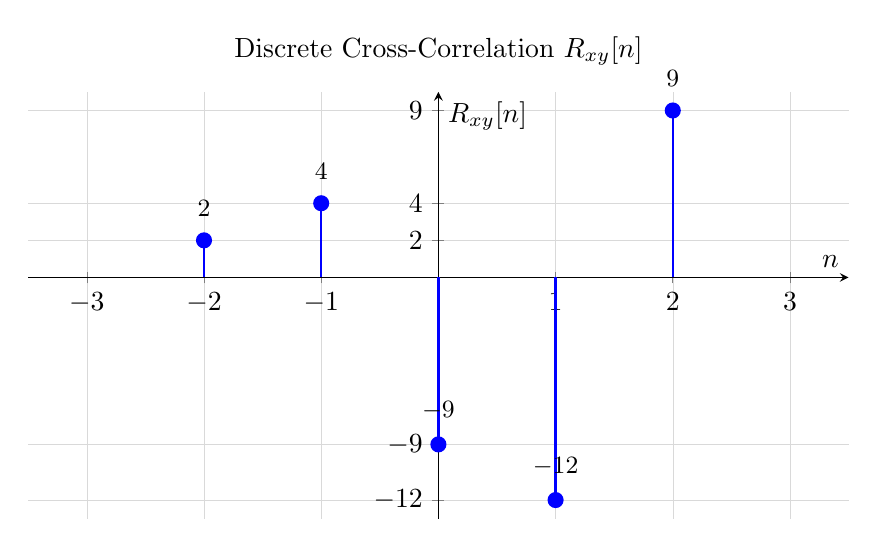
\begin{tikzpicture}
	\pgfplotsset{impulse/.style={ycomb,blue,thick,mark=*,mark size=2.5pt}}
	\begin{axis}[
		width=12cm,
		height=7cm,
		title={Discrete Cross-Correlation $R_{xy}[n]$},
		xlabel={$n$},
		ylabel={$R_{xy}[n]$},
		axis lines=middle,
		xmin=-3.5, xmax=3.5,
		ymin=-13, ymax=10,
		xtick={-3,-2,-1,0,1,2,3},
		ytick={-12, -9, 2, 4, 9},
		grid=major,
		grid style={line width=.1pt, draw=gray!30},
		]
		\addplot[impulse, nodes near coords,
		every node near coord/.style={font=\small,text=black,
			yshift=5pt, anchor=south}]
		coordinates {(-2,2) (-1,4) (0,-9) (1,-12) (2,9)};
	\end{axis}
\end{tikzpicture}